\chapter{Concentric spheres in a uniform electrostatic field}
\label{app:concentric_spheres}
Coating proppant particles with a conductive material is one potential strategy for generating an electrically conductive proppant pack. In this appendix, we work through a derivation of the electric potential outside of two concentric spheres in the presence of a uniform electrostatic field. Using this solution, we estimate an effective electrical conductivity of a composite particle.

\section{Setup}
The set-up is shown in Figure \ref{fig:concentric_sphere_setup}
\begin{itemize}
    \item primary electric field $\mathbf{E_0} = E_0 \hat{x}$
    \item background conductivity $\sigma_0$,
    \item outer shell conductivity $\sigma_1$ and radius $R_1$
    \item inner sphere conductivity $\sigma_2$ and radius $R_2$
\end{itemize}

\begin{figure}[htb!]
    \centering
    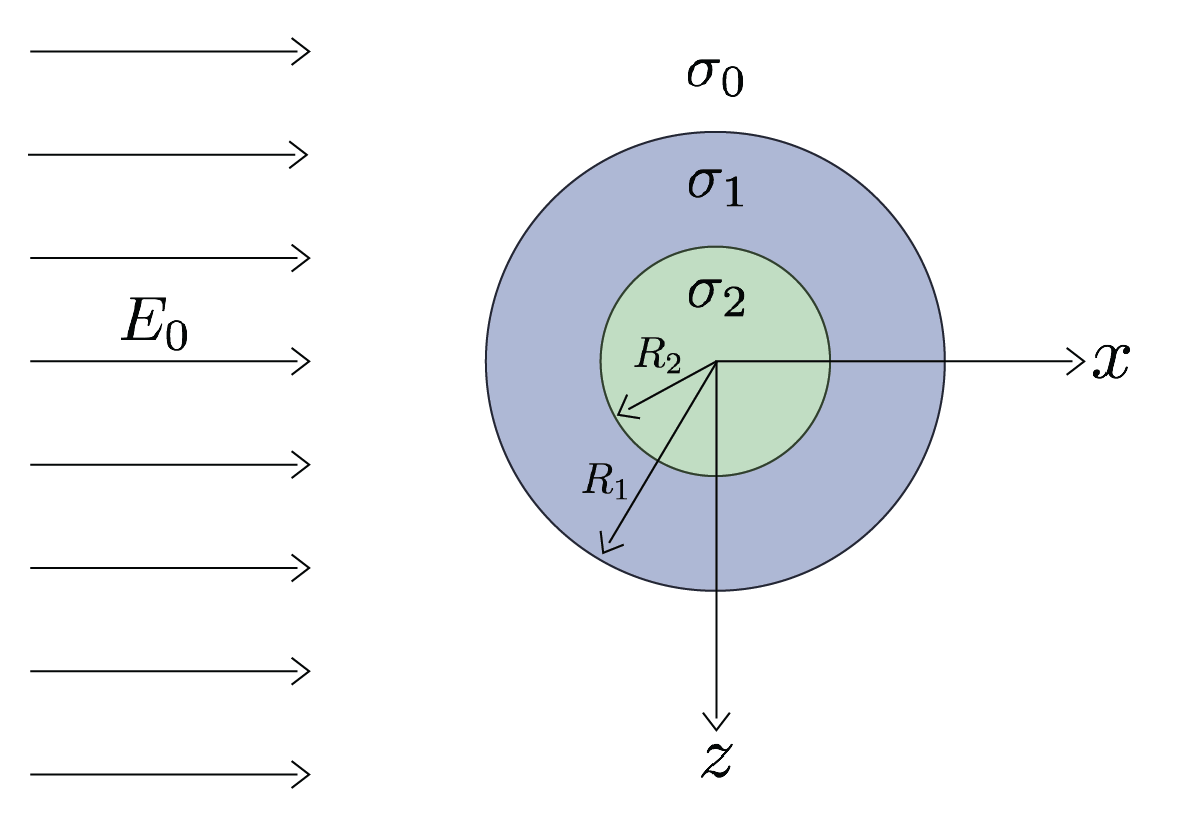
\includegraphics[width=0.6\linewidth]{figures/appendix1/setup}
        \caption{Problem setup. Concentric spheres in a uniform electric field.}
        \label{fig:concentric_sphere_setup}
\end{figure}

The basic equations are
\begin{align}
    \nabla \times \mathbf{E} &= 0  \label{eq:curlE}\\
    \nabla \times \mathbf{H} &= \mathbf{J}\label{eq:curlH}\\
    \mathbf{J} &= \sigma \mathbf{E} \label{eq:JsigE}
\end{align}

By equation \ref{eq:curlE}, we can express $\mathbf{E}$ as a gradient of a potential
    \begin{equation}
        \mathbf{E} = -\nabla V
        \label{eq:V}
    \end{equation}
and combining equations \ref{eq:curlE}, \ref{eq:curlH} and \ref{eq:JsigE}, we see
$$\nabla \times \mathbf{H} = -\sigma \nabla V$$
Taking the divergence gives
$$0 = - \nabla \cdot \sigma \nabla V$$
and in a region with constant $\sigma$
    \begin{equation}
        \nabla^2 V = 0
        \label{eq:laplace}
    \end{equation}

At each of the conductivity interfaces, we have continuity of the normal component of the current density, and continuity of the electric potential. Continuity of the normal current density gives
    \begin{align}
    \sigma_0 \frac{\partial V_0}{\partial r} = \sigma_1 \frac{\partial V_1}{\partial r} \quad \text{at} ~r = R_1 \label{eq:cntsJR1} \\
    \sigma_1 \frac{\partial V_1}{\partial r} = \sigma_2 \frac{\partial V_2}{\partial r} \quad \text{at} ~r = R_2 \label{eq:cntsJR2}
    \end{align}
Continuity of the potential gives
\begin{align}
V_0 = V_1 \quad \text{at} &~r = R_1 \label{eq:cntsVR1}\\
V_1 = V_2 \quad \text{at} &~r = R_2 \label{eq:cntsVR2}
\end{align}


\section{Solving for the Potential}
The primary potential is given by
$$
E_0 \hat{x} = -\frac{\partial V^P}{\partial x} \hat{x} \Rightarrow E_0 = -\frac{\partial V^P}{\partial x}
$$
By integrating in $x$ and setting the reference point to $V^P(r=0) = 0$, we see
    \begin{displaymath}
        \begin{split}
        \int_0^x E_0 dx &= -\int_0^x \frac{\partial V^P}{\partial x} \\
        E_0 x &= -V^P
        \end{split}
    \end{displaymath}
which gives a primary potential of
    \begin{equation}
        V^P = E_0x = E_0 r \cos\theta
    \end{equation}

In spherical coordinates, the Laplace equation, equation \ref{eq:laplace}, is given by
    $$
    \left(\frac{\partial}{\partial r}\left(r^2 \frac{\partial}{\partial r}\right)
    + \frac{1}{\sin \theta}\frac{\partial}{\partial \theta}\left(\sin\theta\frac{\partial}{\partial \theta}\right)
    + \frac{1}{\sin^2\theta} \frac{\partial^2}{\partial \phi^2} \right) V(r,\theta,\phi) = 0
    $$
by symmetry, $V = V(r,\theta)$, so the above equation simplifies to:
    \begin{equation}
    \left(\frac{\partial}{\partial r}\left(r^2 \frac{\partial}{\partial r}\right)
    + \frac{1}{\sin \theta}\frac{\partial}{\partial \theta}\left(\sin\theta\frac{\partial}{\partial \theta}\right)\right) V(r,\theta) = 0
    \label{eq:laplaceSphere}
    \end{equation}
which has general solution
    \begin{equation}
    V = \sum_{n = 0}^{\infty}\left(A_nr^n + \frac{B_n}{r^{n+1}}\right)\text{P}_n(\cos\theta)
    \label{eq:laplaceSphereSoln}
    \end{equation}

\subsection{Solving for the coefficients}

Regarding notation, on the coefficients $A,B$ the subscript denotes the order of the Legendre polynomial and the superscript denotes the region where that coefficient is applicable (i.e. 0: outside the sphere, 1: in the shell, 2: in the inner sphere). On the radius, $R$, the subscript denotes the region (1: outer shell, 2: inner sphere), while the superscript is an exponent.

\subsubsection{Outside the sphere}
Outside the spheres ($r>R_1$), we require that $V\Rightarrow V^P$ for $r \gg R_1$
    $$
    V_0
    = A_0^0
    + A_1^0 r\cos\theta
    + \sum_{n=2}^{\infty} A_n^0 r^n \text{P}_n(\cos\theta)
    + \sum_{n=0}^{\infty} \frac{B_n^0}{r^{n+1}} \text{P}_n(\cos\theta)
    $$
for $r \gg R_1$
    $$
    V_0
    \Rightarrow A_0^0
    + A_1^0 r\cos\theta
    + \sum_{n=2}^{\infty} A_n^0 r^n \text{P}_n(\cos\theta)
    + \sum_{n=0}^{\infty}
    $$
Since the Legendre polynomials, $\text{P}_n(\cos\theta)$, are orthogonal, then $A_0^0, A_n^0 = 0 ~ \forall n$, and $A_1^0 = -E_0$. So
    \begin{mdframed}[backgroundcolor=gray!10, innertopmargin=0pt, innerbottommargin=10pt]
        \begin{equation}
    V_0
    = -E_0 r \cos\theta
    + \sum_{n=0}^{\infty} \frac{B_n^0}{r^{n+1}} \text{P}_n(\cos\theta)
    \label{eq:V0}
    \end{equation}
    \end{mdframed}


\subsubsection{In the outer shell}
In the outer shell ($R_2 < r < R_1$)
\begin{mdframed}[backgroundcolor=gray!10, innertopmargin=0pt, innerbottommargin=10pt]
        \begin{equation}
    V_1
    = \sum_{n = 0}^{\infty}\left(A_n^1r^n + \frac{B_n^1}{r^{n+1}}\right)\text{P}_n(\cos\theta)
        \label{eq:V1}
    \end{equation}
\end{mdframed}
Using the interface condition in equation \ref{eq:cntsVR1}, we have
    \begin{displaymath}
        -E_0 R_1\cos\theta
        + \sum_{n = 0}^{\infty}\left(\frac{B_n^0}{R_1^{n+1}}\right)\text{P}_n(\cos\theta)
        =
        \sum_{n = 0}^{\infty}\left(A_n^1R_1^n + \frac{B_n^1}{R_1^{n+1}}\right)\text{P}_n(\cos\theta)
    \end{displaymath}
    \begin{displaymath}
        \begin{split}
            -E_0 R_1\cos\theta
            + &\frac{B_0^0}{R_1}
            + \frac{B_1^0}{R_1^{2}}\cos\theta
            +\sum_{n = 2}^{\infty}\left(\frac{B_n^0}{R_1^{n+1}}\right)\text{P}_n(\cos\theta)
            \\
            &=
            A_0^1
            + A_1^1R_1\cos\theta
            + \frac{B_0^1}{R_1}
            + \frac{B_1^1}{R_1^{2}}\cos\theta
            + \sum_{n = 2}^{\infty}\left(A_n^1R_1^n + \frac{B_n^1}{R_1^{n+1}}\right)\text{P}_n(\cos\theta)
        \end{split}
    \end{displaymath}
which must hold for all $\theta$. Thus, we can break this up in to a series of smaller equations. For the $n=0$ polynomials, we have
    \begin{equation}
        \begin{split}
        \frac{B_0^0}{R_1} &= A_0^1 + \frac{B_0^1}{R_1} \\
        \Rightarrow \quad
        B_0^0 &= R_1A_0^1 + B_0^1
        \end{split}
        \label{eq:coeff1}
    \end{equation}
For the $n=1$ polynomials, we have
    \begin{equation}
        \begin{split}
        -E_0R_1 + \frac{B_1^0}{R_1^2} &= A_1^1R_1 + \frac{B_1^1}{R_1^2} \\
        \Rightarrow \quad
        -E_0R_1^3 + B_1^0 &= A_1^1R_1^3 + B_1^1
        \end{split}
        \label{eq:coeff2}
    \end{equation}
and for $n\geq 2$ (using orthogonality of $\text{P}_n(\cos\theta)$)
    \begin{equation}
    \begin{split}
        \frac{B_n^0}{R_1^{n+1}} &= A_n^1 R_1^n + \frac{B_n^1}{R_1^{n+1}} \\
        \Rightarrow \quad
        B_n^0 &= A_n^1 R_1^{2n+1} + B_n^1
        \end{split}
        \label{eq:coeff3}
    \end{equation}

Next, we look to the interface conditions on the derivative of the potential, as described in equation \ref{eq:cntsJR1}. We first find the derivatives of $V_0$, $V_1$ with respect to $r$:
    \begin{equation}
        \frac{\partial V_0}{\partial r} = -E_0\cos\theta + \sum_{n=0}^{\infty}-(n+1)\frac{B_n^0}{r^{n+2}}\text{P}_n(\cos\theta)
        \label{eq:dV0dr}
    \end{equation}
    \begin{equation}
        \frac{\partial V_1}{\partial r} = \sum_{n=1}^{\infty}n A_n^{1}r^{n-1}\text{P}_n(\cos\theta) + \sum_{n=0}^{\infty}-(n+1)\frac{B_n^1}{r^{n+2}}\text{P}_n(\cos\theta)
        \label{eq:dV1dr}
    \end{equation}
Imposing the interface in equation \ref{eq:cntsJR1}, we have,
    \begin{displaymath}
        \begin{split}
            -\sigma_0 E_0\cos\theta + \sigma_0 \sum_{n=0}^{\infty}-(n+1)\frac{B_n^0}{R_1^{n+2}}\text{P}_n(\cos\theta)& \\
            = \sigma_1 \sum_{n=1}^{\infty}n A_n^{1}R_1^{n-1}\text{P}_n(\cos\theta) & + \sigma_1 \sum_{n=0}^{\infty}-(n+1)\frac{B_n^1}{R_1^{n+2}}\text{P}_n(\cos\theta)
        \end{split}
    \end{displaymath}
Breaking out coefficients up to $n = 2$ gives
    \begin{displaymath}
        \begin{split}
            - &\sigma_0 E_0\cos\theta
            - \sigma_0 \frac{B_0^0}{R_1^{2}}
            - 2 \sigma_0 \frac{B_1^0}{R_1^{3}}\cos\theta
            - \sigma_0 \sum_{n=2}^{\infty}(n+1)\frac{B_n^0}{R_1^{n+2}}\text{P}_n(\cos\theta) \\
            &= \sigma_1 A_1^1\cos\theta
            - \sigma_1 \frac{B_0^1}{R_1^{2}}
            - 2 \sigma_1 \frac{B_1^1}{R_1^{3}}\cos\theta
            + \sigma_1 \sum_{n=2}^{\infty}\left(nA_n^1R_1^{n-1}-(n+1)\frac{B_n^1}{R_1^{n+2}}\right)\text{P}_n(\cos\theta)
        \end{split}
    \end{displaymath}
Again, this must hold for all $\theta$, so we can break this up into a series of smaller equations. For the $n=0$ polynomials, we have
    \begin{equation}
    \begin{split}
        -\sigma_0 \frac{B_0^0}{R_1^2} &= -\sigma_1\frac{B_0^1}{R_1^2} \\
        \Rightarrow \quad
        \sigma_0 B_0^0 &= \sigma_1 B_0^1
        \end{split}
        \label{eq:coeff4}
    \end{equation}
For the $n=1$ polynomials, we have
    \begin{equation}
        \begin{split}
            - \sigma_0 E_0
            - 2 \sigma_0 \frac{B_1^0}{R_1^{3}}
            &= \sigma_1 A_1^1
            - 2 \sigma_1 \frac{B_1^1}{R_1^{3}} \\
             \Rightarrow \quad
            - \sigma_0 E_0 R_1^{3}
            - 2 \sigma_0 B_1^0
            &= \sigma_1 A_1^1 R_1^{3}
            - 2 \sigma_1 B_1^1
        \end{split}
        \label{eq:coeff5}
    \end{equation}
and for the polynomials where $n \geq 2$, we have
    \begin{equation}
    \begin{split}
            - \sigma_0 (n+1)\frac{B_n^0}{R_1^{n+2}}
            &=
            \sigma_1 nA_n^1R_1^{n-1} - \sigma_1 (n+1)\frac{B_n^1}{R_1^{n+2}}\\
             \Rightarrow \quad
            - \sigma_0 (n+1)B_n^0
            &=
            \sigma_1 nA_n^1R_1^{2n+1} - \sigma_1(n+1)B_n^1
    \end{split}
        \label{eq:coeff6}
    \end{equation}


\subsubsection{Inner sphere}
In the inner-most sphere ($r<R_2$), we have that
    \begin{displaymath}
        V_2 = \sum_{n=0}^{\infty} \left(A_n^2 r^n + \frac{B_n^2}{r^{n+1}}\right) \text{P}_n(\cos\theta)
    \end{displaymath}
as $r \Rightarrow 0$, $V_2 \Rightarrow 0$ by choice of our ref. point. This implies $B_n^2=0 ~ \forall n$, and $A_0^2 = 0$, so we have
\begin{mdframed}[backgroundcolor=gray!10, innertopmargin=0pt, innerbottommargin=10pt]
    \begin{equation}
        V_2 = \sum_{n=1}^{\infty} A_n^2 r^n \text{P}_n(\cos\theta)
        \label{eq:V2}
    \end{equation}
\end{mdframed}
Now we use the interface conditions at $r = R_2$, given by equations \ref{eq:cntsJR2} and \ref{eq:cntsVR2}. Starting with the continuity of the potential $V$ (equation \ref{eq:cntsVR2}), we see
    $$
        \sum_{n = 0}^{\infty}\left(A_n^1r^n + \frac{B_n^1}{r^{n+1}}\right)\text{P}_n(\cos\theta)
        =
        \sum_{n=1}^{\infty} A_n^2 r^n \text{P}_n(\cos\theta)
    $$
which must hold for all $\theta$, giving
    \begin{equation}
        \begin{split}
        A_0^1 + \frac{B_0^1}{R_2}
        &=
        0 \\
        \Rightarrow \quad
        A_0^1R_2 + B_0^1 &= 0
        \end{split}
        \label{eq:coeff7}
    \end{equation}
and for $n \geq 1$,
    \begin{equation}
    \begin{split}
        A_n^1R_2^n + \frac{B_n^1}{R_2^{n+1}}
        &=
        A_n^2 R_2^n \\
        \Rightarrow \quad
        A_n^1R_2^{2n+1} + B_n^1
        &=
        A_n^2 R_2^{2n+1}
        \end{split}
        \label{eq:coeff8}
    \end{equation}
For the continuity of the current density (equation \ref{eq:cntsJR2}), we have
    $$
        \sigma_1 \sum_{n=1}^\infty n A_n^1 R_2^{n-1}\text{P}_n(\cos\theta)
        - \sigma_1 \sum_{n=0}^\infty (n+1)\frac{B_n^1}{R_2^{n+2}} \text{P}_n(\cos\theta)
        =
        \sigma_2 \sum_{n=1}^\infty n A_n^2 R_2^{n-1}\text{P}_n(\cos\theta)
    $$
which must hold for all $\theta$, giving
    \begin{displaymath}
        -\sigma_1 \frac{B_0^1}{R_2} = 0
    \end{displaymath}
and since both $\sigma_1$ and $R_2$ are non-zero,
    \begin{mdframed}[backgroundcolor=gray!10, innertopmargin=0pt, innerbottommargin=10pt]
    \begin{equation}
        B_0^1 = 0
        \label{eq:coeff9}
    \end{equation}
    \end{mdframed}
and for $n \geq 1$
    \begin{equation}
    \begin{split}
        \sigma_1 n A_n^1 R_2^{n-1}
        - \sigma_1 (n+1)\frac{B_n^1}{R_2^{n+2}}
        &=
        \sigma_2 n A_n^2 R_2^{n-1} \\
        \Rightarrow \quad
        \sigma_1 n A_n^1 R_2^{2n+1}
        - \sigma_1 (n+1)B_n^1
        &=
        \sigma_2 n A_n^2 R_2^{2n+1}
        \end{split}
        \label{eq:coeff10}
    \end{equation}

Now that we have equations \ref{eq:coeff1}, \ref{eq:coeff2}, \ref{eq:coeff3}, \ref{eq:coeff4}, \ref{eq:coeff5}, \ref{eq:coeff6}, \ref{eq:coeff7}, \ref{eq:coeff8}, \ref{eq:coeff9} and \ref{eq:coeff10}, we have 10 equations and 10 unknowns. Therefore, we can proceed to solve for each of the coefficients.

By combining \ref{eq:coeff7} and \ref{eq:coeff9}, we see
\begin{mdframed}[backgroundcolor=gray!10, innertopmargin=0pt, innerbottommargin=10pt]
\begin{equation}
    A_0^1 = 0.
    \label{eq:coeff11}
\end{equation}
\end{mdframed}
Combining this with equation \ref{eq:coeff1}, we see
\begin{mdframed}[backgroundcolor=gray!10, innertopmargin=0pt, innerbottommargin=10pt]
\begin{equation}
    B_0^0 = 0
    \label{eq:coeff12}
\end{equation}
\end{mdframed}
From equation \ref{eq:coeff2}, we know $B_1^1 = -E_0R_1^3 + B_1^0 - A_1^1R_1^3$, which we put into equation \ref{eq:coeff5} to give
\begin{displaymath}
    - \sigma_0 E_0 R_1^{3}
    - 2 \sigma_0 B_1^0
    = \sigma_1 A_1^1 R_1^{3}
    - 2 \sigma_1 (-E_0R_1^3 + B_1^0 - A_1^1R_1^3)
\end{displaymath}
giving us an equation in $A_1^1$ and $B_1^0$, which we can simplify to
\begin{equation}
    - E_0 R_1^{3} (\sigma_0 + 2\sigma_1)
    = 3\sigma_1 A_1^1 R_1^{3}
    + 2 (\sigma_0-\sigma_1)B_1^0
    \label{eq:coeff13}
\end{equation}
From equation \ref{eq:coeff8}, we know $ A_n^2 R_2^{2n+1}= A_n^1R_2^{2n+1} + B_n^1.$ Putting this in to eqn \ref{eq:coeff10}, we see
\begin{displaymath}
    \sigma_1 n A_n^1 R_2^{2n+1}
    - \sigma_1 (n+1)B_n^1
    =
    \sigma_2 n (A_n^1R_2^{2n+1} + B_n^1) \quad n \geq 1
\end{displaymath}
which simplifies to
\begin{equation}
    n(\sigma_1 - \sigma_2)  A_n^1 R_2^{2n+1}
    =
    ((n+1)\sigma_1  + n\sigma_2 ) B_n^1 R_2^{2n+1} \quad n \geq 1
    \label{eq:coeff14}
\end{equation}
In the case where $n=1$, we have that
\begin{equation}
    \begin{split}
        (\sigma_1 - \sigma_2) A_1^1 R_2^{3}
        &=
        (2\sigma_1 + \sigma_2) B_1^1 \\
        \Rightarrow \quad
         A_1^1
        &=
        \left(\frac{2\sigma_1 + \sigma_2}{\sigma_1 - \sigma_2}\right) \frac{B_1^1}{R_2^{3}}
    \end{split}
    \label{eq:starstar}
\end{equation}
which we can put into equation \ref{eq:coeff13} giving
\begin{equation}
    - (\sigma_0 + 2\sigma_1)E_0 R_1^{3}
    = 3\sigma_1 \left(\frac{2\sigma_1 + \sigma_2}{\sigma_1 - \sigma_2}\right) \left(\frac{R_1 }{R_2}\right)^3 B_1^1
    + 2 (\sigma_0-\sigma_1)B_1^0
    \label{eq:coeff15}
\end{equation}
To get another equation in $B_1^0$ and $B_1^1$, we use equations \ref{eq:coeff2} and \ref{eq:starstar} to get
\begin{displaymath}
    \begin{split}
        B_1^1 = -E_0R_1^3 + B_1^0 - \left(\frac{2\sigma_1 + \sigma_2}{\sigma_1 - \sigma_2}\right) \left(\frac{R_1}{R_2}\right)^3 B_1^1 \\
        \Rightarrow \quad
         \left(1+ \left(\frac{2\sigma_1 + \sigma_2}{\sigma_1 - \sigma_2}\right) \left(\frac{R_1}{R_2}\right)^3\right) B_1^1 = -E_0R_1^3 + B_1^0
    \end{split}
\end{displaymath}
to ease notation, define
\begin{equation}
    \alpha = \left(\frac{R_1}{R_2}\right)^3
    \label{eq:alpha}
\end{equation}
which lets us simplify the above to
\begin{equation}
    \begin{split}
         B_1^1 &= \left(-E_0 R_1^3 + B_1^0\right)\left(1+ \left(\frac{2\sigma_1 + \sigma_2}{\sigma_1 - \sigma_2}\right) \alpha \right)^{-1}
         \\
         &= \left(-E_0 R_1^3 + B_1^0\right)\left(\frac{\left(\sigma_1 - \sigma_2\right) + \left(2\sigma_1 + \sigma_2\right)\alpha}{\sigma_1 - \sigma_2}  \right)^{-1}
         \\
         &= \left(-E_0 R_1^3 + B_1^0\right)\left(\frac{\sigma_1 - \sigma_2} {\left(\sigma_1 - \sigma_2\right) + \left(2\sigma_1 + \sigma_2\right)\alpha} \right)
     \end{split}
     \label{eq:coeff16}
\end{equation}
With equations \ref{eq:coeff15} and \ref{eq:coeff16}, we finally have arrived at a set of two equations with two unknowns ($B_1^1$ and ($B_1^0$). Putting equation \ref{eq:coeff16} into equation \ref{eq:coeff15} and using the definition of $\alpha$ as given in equation \ref{eq:alpha}, we see
\begin{displaymath}
    \begin{split}
    & - (\sigma_0 + 2\sigma_1)E_0 R_1^{3}
    \\ & \quad\quad
    =
    3\sigma_1\alpha \left(\frac{2\sigma_1 + \sigma_2}{\sigma_1 - \sigma_2}\right) \left(\frac{\sigma_1 - \sigma_2} {\left(\sigma_1 - \sigma_2\right) + \left(2\sigma_1 + \sigma_2\right)\alpha} \right)(-E_0 R_1^3 + B_1^0)
    + 2 (\sigma_0-\sigma_1)B_1^0
    \\
    & \Rightarrow
    - (\sigma_0 + 2\sigma_1)E_0 R_1^{3}
    \\ & \quad\quad
    =
    3\sigma_1\alpha\left(\frac{2\sigma_1 + \sigma_2} {(\sigma_1 - \sigma_2) + (2\sigma_1 + \sigma_2)\alpha} \right) (-E_0 R_1^3 + B_1^0)
    + 2 (\sigma_0-\sigma_1)B_1^0
    \\
    & \Rightarrow
    - (\sigma_0 + 2\sigma_1)E_0 R_1^{3}
    \\ & \quad\quad
     =
    \left(\frac{3\sigma_1(2\sigma_1 + \sigma_2)\alpha} {(\sigma_1 - \sigma_2) + (2\sigma_1 + \sigma_2)\alpha} \right)(-E_0 R_1^3 + B_1^0)
    + 2 (\sigma_0-\sigma_1)B_1^0
    \\
    & \Rightarrow
    -\left( (\sigma_0 + 2\sigma_1) - \frac{3\sigma_1(2\sigma_1 + \sigma_2)\alpha} {(\sigma_1 - \sigma_2) + (2\sigma_1 + \sigma_2)\alpha}\right)
    E_0 R_1^{3}
    \\ & \quad\quad
     =
    \left(\frac{3\sigma_1(2\sigma_1 + \sigma_2)\alpha} {(\sigma_1 - \sigma_2) + (2\sigma_1 + \sigma_2)\alpha} + 2 (\sigma_0-\sigma_1) \right)
    B_1^0
    \\
    & \Rightarrow
    -\left(
    \frac{(\sigma_0 + 2\sigma_1)(\sigma_1 - \sigma_2) + (\sigma_0 + 2\sigma_1)(2\sigma_1 + \sigma_2)\alpha- 3\sigma_1(2\sigma_1 + \sigma_2)\alpha}
    {(\sigma_1 - \sigma_2) + (2\sigma_1 + \sigma_2)\alpha}
    \right)
    E_0 R_1^{3}
    \\ & \quad\quad
     =
    \left(
    \frac{3\sigma_1(2\sigma_1 + \sigma_2)\alpha + 2 (\sigma_0-\sigma_1)(\sigma_1 - \sigma_2) + 2 (\sigma_0-\sigma_1)(2\sigma_1 + \sigma_2)\alpha}
    {(\sigma_1 - \sigma_2) + (2\sigma_1 + \sigma_2)\alpha}
    \right)
    B_1^0
    \\
    & \Rightarrow
    -\left(
    (\sigma_0 + 2\sigma_1)(\sigma_1 - \sigma_2) + (\sigma_0 - \sigma_1)(2\sigma_1 + \sigma_2)\alpha
    \right)
    E_0 R_1^{3}
    \\ & \quad\quad
    =
    \left(
    2 (\sigma_0-\sigma_1)(\sigma_1 - \sigma_2) + (2\sigma_0 + \sigma_1)(2\sigma_1 + \sigma_2)\alpha
    \right)
    B_1^0
    \end{split}
\end{displaymath}
So the coefficient $B_1^0$ is given by
\begin{mdframed}[backgroundcolor=gray!10, innertopmargin=0pt, innerbottommargin=10pt]
\begin{equation}
    B_1^0
     =
    -E_0 R_1^{3}
    \left(
    \frac{
    (\sigma_0 + 2\sigma_1)(\sigma_1 - \sigma_2) + (\sigma_0 - \sigma_1)(2\sigma_1 + \sigma_2)\alpha
    }
    {
    2 (\sigma_0-\sigma_1)(\sigma_1 - \sigma_2) + (2\sigma_0 + \sigma_1)(2\sigma_1 + \sigma_2)\alpha
    }
    \right)
    \label{eq:B10}
\end{equation}
\end{mdframed}
Putting this into equation \ref{eq:coeff16}, we can solve for $B_1^1$
\begin{displaymath}
    \begin{split}
    & B_1^1 =
        -E_0 R_1^3\left( 1 +
    \frac{
    (\sigma_0 + 2\sigma_1)(\sigma_1 - \sigma_2) + (\sigma_0 - \sigma_1)(2\sigma_1 + \sigma_2)\alpha
    }
    {
    2 (\sigma_0-\sigma_1)(\sigma_1 - \sigma_2) + (2\sigma_0 + \sigma_1)(2\sigma_1 + \sigma_2)\alpha
    }
    \right) \\
        & \quad\quad\quad\quad\quad\quad\quad \left(
        \frac{\sigma_1 - \sigma_2} {\left(\sigma_1 - \sigma_2\right) + \left(2\sigma_1 + \sigma_2\right)\alpha}
        \right)
    \\
    \Rightarrow
    &B_1^1 =
    -E_0 R_1^3\left(
    \frac{
    3 \sigma_0(\sigma_1 - \sigma_2) + 3\sigma_0(2\sigma_1 + \sigma_2)\alpha
    }
    {
    2 (\sigma_0-\sigma_1)(\sigma_1 - \sigma_2) + (2\sigma_0 + \sigma_1)(2\sigma_1 + \sigma_2)\alpha
    }
    \right)
    \\ & \quad\quad\quad\quad\quad\quad\quad
        \left(
        \frac{\sigma_1 - \sigma_2} {\left(\sigma_1 - \sigma_2\right) + \left(2\sigma_1 + \sigma_2\right)\alpha}
        \right)
    \end{split}
\end{displaymath}
\begin{mdframed}[backgroundcolor=gray!10, innertopmargin=0pt, innerbottommargin=10pt]
\begin{equation}
    B_1^1
    =
    -E_0 R_1^3 \left(
    \frac{
    3 \sigma_0 (\sigma_1 - \sigma_2)
    }
    {
    2 (\sigma_0-\sigma_1)(\sigma_1 - \sigma_2) + (2\sigma_0 + \sigma_1)(2\sigma_1 + \sigma_2)\alpha
    }
    \right)
    \label{eq:B11}
\end{equation}
\end{mdframed}
Next, we solve for $A_1^1$ using equation \ref{eq:starstar}.
\begin{displaymath}
\begin{split}
    A_1^1
        &=
        \left(\frac{2\sigma_1 + \sigma_2}{\sigma_1 - \sigma_2}\right) \frac{1}{R_2^3}
        \left(
        -E_0 R_1^3 \left(
        \frac{
        3 \sigma_0 (\sigma_1 - \sigma_2)
        }
        {
        2 (\sigma_0-\sigma_1)(\sigma_1 - \sigma_2) + (2\sigma_0 + \sigma_1)(2\sigma_1 + \sigma_2)\alpha
        }
        \right)
        \right)
\end{split}
\end{displaymath}
which simplifies to
\begin{mdframed}[backgroundcolor=gray!10, innertopmargin=0pt, innerbottommargin=10pt]
    \begin{equation}
        A_1^1=
        -E_0 \alpha \left(
        \frac{
        3 \sigma_0 (2\sigma_1 + \sigma_2)
        }
        {
        2 (\sigma_0-\sigma_1)(\sigma_1 - \sigma_2) + (2\sigma_0 + \sigma_1)(2\sigma_1 + \sigma_2)\alpha
        }
        \right)
        \label{eq:A11}
    \end{equation}
\end{mdframed}
Now, using equation \ref{eq:coeff10} for $n=1$, we can solve for $A_1^2$
\begin{displaymath}
    \begin{split}
        \sigma_2  A_1^2 R_2^3
        & =
        \sigma_1 A_1^1 R_2^3
        - 2 \sigma_1 B_1^1
        \\
        A_1^2
        & =
        \frac{\sigma_1}{\sigma_2}
        \left(
         A_1^1
        - \frac{2}{R_2^3} B_1^1
        \right)
        \\
        & =
        -E_0 \alpha \frac{\sigma_1}{\sigma_2}
         \left(
        \frac{
        3 \sigma_0 (2\sigma_1 + \sigma_2) - 2 (3 \sigma_0 (\sigma_1 - \sigma_2))
        }
        {
        2 (\sigma_0-\sigma_1)(\sigma_1 - \sigma_2) + (2\sigma_0 + \sigma_1)(2\sigma_1 + \sigma_2)\alpha
        }
        \right)
        \\
        & =
        -E_0 \alpha \frac{\sigma_1}{\sigma_2}
         \left(
        \frac{
        3 \sigma_0 (3\sigma_2)
        }
        {
        2 (\sigma_0-\sigma_1)(\sigma_1 - \sigma_2) + (2\sigma_0 + \sigma_1)(2\sigma_1 + \sigma_2)\alpha
        }
        \right)
    \end{split}
\end{displaymath}
\begin{mdframed}[backgroundcolor=gray!10, innertopmargin=0pt, innerbottommargin=10pt]
\begin{equation}
        A_1^2
        =
        -E_0 \alpha
         \left(
        \frac{
        3 \sigma_0 (3\sigma_1)
        }
        {
        2 (\sigma_0-\sigma_1)(\sigma_1 - \sigma_2) + (2\sigma_0 + \sigma_1)(2\sigma_1 + \sigma_2)\alpha
        }
        \right)
        \label{eq:A12}
\end{equation}
\end{mdframed}

At this point, the remaining coefficients to be found are $B_n^0$, $A_n^1$ and $B_n^1$ and $A_n^2$ for $n \geq 2$, and four remaining equations \ref{eq:coeff3}, \ref{eq:coeff6}, \ref{eq:coeff8} and \ref{eq:coeff10} for each $n$. These can be written more concisely as a matrix equation, namely
\begin{equation}
    \left(
    \begin{array}{c}
        0 \\
        0 \\
        0 \\
        0
    \end{array}
    \right)
    =
    \left(
    \begin{array}{cccc}
        1          & 0        & -1            & 1              \\
        n\sigma_1  & 0        & (n+1)\sigma_0 & -(n+1)\sigma_1 \\
        1          & -1       & 0             & 1              \\
        n \sigma_1 & -n\sigma_2 & 0             & -(n+1)\sigma_1
    \end{array}
    \right)
    \left(
    \begin{array}{c}
        A_n^1 R_1^{2n+1} \\
        B_n^0            \\
        A_n^2 R_2^{2n+1} \\
        B_n^1            \\
    \end{array}
    \right)
    \label{eq:matrixeqn}
\end{equation}
The solution to equation \ref{eq:matrixeqn} requires the matrix inverse. If the matrix is invertible, than the unique solution is $(0,0,0,0)$. To test if this is invertible, we perform Gaussian elimination to try and reduce it to the identity:
\begin{displaymath}
    \begin{split}
    &\left(
    \begin{array}{cccc}
        1          & 0        & -1            & 1              \\
        1          & -1       & 0             & 1              \\
        n \sigma_1 & -n\sigma_2 & 0           & -(n+1)\sigma_1 \\
        n\sigma_1  & 0        & (n+1)\sigma_0 & -(n+1)\sigma_1 \\
    \end{array}
    \right)
    \\
    &\sim
    \left(
    \begin{array}{cccc}
        1          & 0          & -1                       & 1              \\
        0          & -1         & 0                        & 1              \\
        0          & 0          & (n+1)\sigma_0 +n\sigma_1 & -(2n+1)\sigma_1\\
        0          & -n\sigma_2 & n\sigma_1                & -(2n+1)\sigma_1 \\
    \end{array}
    \right)
    \\
    \end{split}
\end{displaymath}
\begin{displaymath}
    \begin{split}
        &\sim
    \left(
    \begin{array}{cccc}
        1          & 0          & -1                       & 1               \\
        0          & 1          & 0                        & -1              \\
        0          & 0          & (n+1)\sigma_0 +n\sigma_1 & -(2n+1)\sigma_1 \\
        0          & 0          & n\sigma_1                & -(2n+1)\sigma_1 -n\sigma_2 \\
    \end{array}
    \right)
    \\
        &\sim
    \left(
    \begin{array}{cccc}
        1          & 0          & -1                       & 1               \\
        0          & 1          & 0                        & -1              \\
        0          & 0          & 1                        & \frac{-(2n+1)\sigma_1}{(n+1)\sigma_0 +n\sigma_1} \\
        0          & 0          & 0                        & -(2n+1)\sigma_1 -n\sigma_2 - n\sigma_1\frac{-(2n+1)\sigma_1}{(n+1)\sigma_0 +n\sigma_1}  \\
    \end{array}
    \right)
    \\
        &\sim
    \left(
    \begin{array}{cccc}
        1          & 0          & -1                       & 1               \\
        0          & 1          & 0                        & -1              \\
        0          & 0          & 1                        & \frac{-(2n+1)\sigma_1}{(n+1)\sigma_0 +n\sigma_1} \\
        0          & 0          & 0                        & 1  \\
    \end{array}
    \right)
    \\
        &\sim
    \left(
    \begin{array}{cccc}
        1          & 0          & 0                        & 0 \\
        0          & 1          & 0                        & 0 \\
        0          & 0          & 1                        & 0 \\
        0          & 0          & 0                        & 1  \\
    \end{array}
    \right)
    \end{split}
\end{displaymath}
Therefore,
\begin{mdframed}[backgroundcolor=gray!10, innertopmargin=0pt, innerbottommargin=10pt]
\begin{equation}
    A_n^1 = 0 \quad \forall n \geq 2
    \label{eq:An1}
\end{equation}
\end{mdframed}
\begin{mdframed}[backgroundcolor=gray!10, innertopmargin=0pt, innerbottommargin=10pt]
\begin{equation}
    B_n^0 = 0 \quad \forall n \geq 2
    \label{eq:Bn0}
\end{equation}
\end{mdframed}
\begin{mdframed}[backgroundcolor=gray!10, innertopmargin=0pt, innerbottommargin=10pt]
\begin{equation}
    A_n^2 = 0 \quad \forall n \geq 2
    \label{eq:An2}
\end{equation}
\end{mdframed}
\begin{mdframed}[backgroundcolor=gray!10, innertopmargin=0pt, innerbottommargin=10pt]
\begin{equation}
    B_n^1 = 0 \quad \forall n \geq 2
    \label{eq:Bn1}
\end{equation}
\end{mdframed}

Now we have everything we need to express the potentials in each region. Outside the sphere ($r > R_2$)
    \begin{mdframed}[backgroundcolor=gray!10, innertopmargin=0pt, innerbottommargin=10pt]
        \begin{equation}
    V_0
    = -E_0 r \cos\theta
    \left(1+
    \frac{R_1^{3}}{r^3}
    \left(
    \frac{
    (\sigma_0 + 2\sigma_1)(\sigma_1 - \sigma_2) + (\sigma_0 - \sigma_1)(2\sigma_1 + \sigma_2)\alpha
    }
    {
    2 (\sigma_0-\sigma_1)(\sigma_1 - \sigma_2) + (2\sigma_0 + \sigma_1)(2\sigma_1 + \sigma_2)\alpha
    }
    \right)\right)
    \label{eq:V0final}
    \end{equation}
    \end{mdframed}
In the outer shell ($R_1<r<R_2$)
\begin{mdframed}[backgroundcolor=gray!10, innertopmargin=0pt, innerbottommargin=10pt]
    \begin{equation}
    \begin{split}
    V_1
    =
    -E_0r\cos\theta\frac{3\sigma_0}{2 (\sigma_0-\sigma_1)(\sigma_1 - \sigma_2) + (2\sigma_0 + \sigma_1)(2\sigma_1 + \sigma_2)\alpha}
    \\ \left(
            (2\sigma_1 + \sigma_2)\alpha +
             (\sigma_1 - \sigma_2) \frac{R_1^3}{r^3}
    \right)
    \end{split}
    \label{eq:V1final}
    \end{equation}
\end{mdframed}
In the inner sphere ($r<R_2$)
\begin{mdframed}[backgroundcolor=gray!10, innertopmargin=0pt, innerbottommargin=10pt]
    \begin{equation}
        V_2
        % =\sum_{n=1}^{\infty} A_n^2 r^n \text{P}_n(\cos\theta)
        =-E_0 r\cos\theta
         \left(
        \frac{
        (3 \sigma_0) (3\sigma_1)\alpha
        }
        {
        2 (\sigma_0-\sigma_1)(\sigma_1 - \sigma_2) + (2\sigma_0 + \sigma_1)(2\sigma_1 + \sigma_2)\alpha
        }
        \right)
        \label{eq:V2final}
    \end{equation}
\end{mdframed}


\subsection{Sanity Checks}
Before moving any further, there are a few end-member cases we can use to validate our solution.

For a number of checks, it is useful to compare to the solution of a single sphere. From Ward and Hohmann (pg. 282-285), we have that the potential exterior to the sphere ($r > R$) is
\begin{equation}
    V_e = -E_0 r \cos \theta \left(1 + \frac{R^3}{r^3}\left(\frac{\sigma_e-\sigma_i}{2\sigma_e+\sigma_i}\right)\right)
    \label{eq:Ve}
\end{equation}
where $\sigma_e$ is the conductivity of the background, $\sigma_i$ is the conductivity of the sphere, and $R$ is the radius of the sphere. The potential inside the sphere ($r < R$) is given by
\begin{equation}
    V_i = -E_0r\cos\theta\left(\frac{3\sigma_e}{2\sigma_e+\sigma_i}\right)
    \label{eq:Vi}
\end{equation}

\subsubsection{Check 1: Equal conductivity of the inner sphere and outer shell}
First, if $\sigma_2 = \sigma_1$, then $R=R_1$, and we expect $V_0=V_e$ and $V_1=V_2=V_i$. Starting with $V_0$, we see
\begin{displaymath}
    \begin{split}
    V_0
    &= -E_0 r \cos\theta
    \left(1+
    \frac{R_1^{3}}{r^3}
    \left(
    \frac{
    (\sigma_0 + 2\sigma_1)(\sigma_1 - \sigma_1) + (\sigma_0 - \sigma_1)(2\sigma_1 + \sigma_1)\alpha
    }
    {
    2 (\sigma_0-\sigma_1)(\sigma_1 - \sigma_1) + (2\sigma_0 + \sigma_1)(2\sigma_1 + \sigma_1)\alpha
    }
    \right)\right)
    \\
        &= -E_0 r \cos\theta
    \left(1+
    \frac{R_1^{3}}{r^3}
    \left(
    \frac{
    (\sigma_0 - \sigma_1)(3\sigma_1)\alpha
    }
    {
    (2\sigma_0 + \sigma_1)(3\sigma_1)\alpha
    }
    \right)\right)
    \\
    &= -E_0 r \cos\theta
    \left(1+
    \frac{R_1^{3}}{r^3}
    \left(
    \frac{
    \sigma_0 - \sigma_1
    }
    {
    2\sigma_0 + \sigma_1
    }
    \right)\right)
    \\
    &= V_e ~\checkmark
    \end{split}
\end{displaymath}
For $V_1$, we have
\begin{displaymath}
    \begin{split}
    V_1
    &=
    -E_0r\cos\theta\frac{3\sigma_0}{2 (\sigma_0-\sigma_1)(\sigma_1 - \sigma_1) + (2\sigma_0 + \sigma_1)(2\sigma_1 + \sigma_1)\alpha}
    \\&\quad\quad\quad\quad\quad\quad\quad\quad\quad\quad\quad\quad\quad\left(
            (2\sigma_1 + \sigma_1)\alpha +
             (\sigma_1 - \sigma_1) \frac{R_1^3}{r^3}
    \right)
    \\
    &=
    -E_0r\cos\theta\frac{3\sigma_0}{(2\sigma_0 + \sigma_1)(3\sigma_1)\alpha}
    \left(
            (3\sigma_1)\alpha
    \right)
    \\
    &=
    -E_0r\cos\theta\frac{3\sigma_0}{(2\sigma_0 + \sigma_1)}
    \\
    &=
    V_i ~\checkmark
    \end{split}
\end{displaymath}
For $V_2$, we have
\begin{displaymath}
    \begin{split}
        V_2
        &=-E_0 r\cos\theta
         \left(
        \frac{
        (3 \sigma_0) (3\sigma_1)\alpha
        }
        {
        2 (\sigma_0-\sigma_1)(\sigma_1 - \sigma_1) + (2\sigma_0 + \sigma_1)(2\sigma_1 + \sigma_1)\alpha
        }
        \right)
        \\
        &=-E_0 r\cos\theta
         \left(
        \frac{
        (3 \sigma_0) (3\sigma_1)\alpha
        }
        {
        (2\sigma_0 + \sigma_1)(3\sigma_1)\alpha
        }
        \right)
        \\
            &=-E_0 r\cos\theta
         \left(
        \frac{
        3 \sigma_0
        }
        {
        2\sigma_0 + \sigma_1
        }
        \right)
        \\
        &=
        V_i ~\checkmark
    \end{split}
\end{displaymath}

\subsubsection{Check 2: Conductivity of the outer shell equals that of the background}
If $\sigma_1=\sigma_0$, then $R=R_2$, and we expect $V_0 = V_1= V_e$ and $V_2 = V_i$. For $V_0$, we have
\begin{displaymath}
    \begin{split}
    V_0
    &= -E_0 r \cos\theta
    \left(1+
    \frac{R_1^{3}}{r^3}
    \left(
    \frac{
    (\sigma_0 + 2\sigma_0)(\sigma_0 - \sigma_2) + (\sigma_0 - \sigma_0)(2\sigma_0 + \sigma_2)\alpha
    }
    {
    2 (\sigma_0-\sigma_0)(\sigma_0 - \sigma_2) + (2\sigma_0 + \sigma_0)(2\sigma_0 + \sigma_2)\alpha
    }
    \right)\right)
    \\
    &= -E_0 r \cos\theta
    \left(1+
    \frac{R_1^{3}}{r^3}
    \left(
    \frac{
    (3\sigma_0)(\sigma_0 - \sigma_2)
    }
    {
    (3\sigma_0)(2\sigma_0 + \sigma_2)\alpha
    }
    \right)\right)
    \\
    &= -E_0 r \cos\theta
    \left(1+
    \frac{R_1^{3}}{r^3}
    \left(
    \frac{
    (\sigma_0 - \sigma_2)
    }
    {
    (2\sigma_0 + \sigma_2)\alpha
    }
    \right)\right)
    \\
    &= -E_0 r \cos\theta
    \left(1+
    \frac{R_1^{3}}{r^3}
    \left(
    \frac{
    \sigma_0 - \sigma_2
    }
    {
    2\sigma_0 + \sigma_2
    }\right)
    \frac{R_2^3}{R_1^3}
    \right)
    \\
    &= -E_0 r \cos\theta
    \left(1+
    \frac{R_2^{3}}{r^3}
    \left(
    \frac{
    \sigma_0 - \sigma_2
    }
    {
    2\sigma_0 + \sigma_2
    }
    \right)\right)
    \\
    &= V_e ~\checkmark
    \end{split}
 \end{displaymath}
 For $V_1$, we have
 \begin{displaymath}
    \begin{split}
    V_1
    &=
    -E_0r\cos\theta\frac{3\sigma_0}{2 (\sigma_0-\sigma_0)(\sigma_0 - \sigma_2) + (2\sigma_0 + \sigma_0)(2\sigma_0 + \sigma_2)\alpha}
    \\& \quad\quad\quad\quad\quad\quad\quad\quad\quad\quad\quad\quad \left(
            (2\sigma_0 + \sigma_2)\alpha +
             (\sigma_0 - \sigma_2) \frac{R_1^3}{r^3}
    \right)
    \\
        &=
    -E_0r\cos\theta\frac{3\sigma_0}{(3\sigma_0)(2\sigma_0 + \sigma_2)\alpha}
    \left(
            (2\sigma_0 + \sigma_2)\alpha +
             (\sigma_0 - \sigma_2) \frac{R_1^3}{r^3}
    \right)
    \\
        &=
    -E_0r\cos\theta\frac{1}{(2\sigma_0 + \sigma_2)\alpha}
    \left(
            (2\sigma_0 + \sigma_2)\alpha +
             (\sigma_0 - \sigma_2) \frac{R_1^3}{r^3}
    \right)
    \\
            &=
    -E_0r\cos\theta
    \left(
            1 +
             \left(\frac{\sigma_0 - \sigma_2}{(2\sigma_0 + \sigma_2)\alpha} \right) \frac{R_1^3}{r^3}
    \right)
    \\
    &=
    -E_0r\cos\theta
    \left(
            1 +
             \left(\frac{\sigma_0 - \sigma_2}{2\sigma_0 + \sigma_2} \right)\frac{R_2^3}{R_1^3} \frac{R_1^3}{r^3}
    \right)
    \\
        &=
    -E_0r\cos\theta
    \left(
            1 +
             \left(\frac{\sigma_0 - \sigma_2}{2\sigma_0 + \sigma_2} \right)\frac{R_2^3}{r^3}
    \right)
    \\
    &=
    V_e ~\checkmark
    \end{split}
 \end{displaymath}
and for $V_2$,
\begin{displaymath}
    \begin{split}
        V_2
        &=-E_0 r\cos\theta
         \left(
        \frac{
        (3 \sigma_0) (3\sigma_0)\alpha
        }
        {
        2 (\sigma_0-\sigma_0)(\sigma_0 - \sigma_2) + (2\sigma_0 + \sigma_0)(2\sigma_0 + \sigma_2)\alpha
        }
        \right)
        \\
        &=-E_0 r\cos\theta
         \left(
        \frac{
        (3 \sigma_0) (3\sigma_0)\alpha
        }
        {
        (3\sigma_0)(2\sigma_0 + \sigma_2)\alpha
        }
        \right)
        \\
        &=-E_0 r\cos\theta
         \left(
        \frac{
        3 \sigma_0
        }
        {
        2\sigma_0 + \sigma_2
        }
        \right)
        \\
        &=V_i ~\checkmark
    \end{split}
\end{displaymath}

\subsubsection{Check 3: Equal radius of the inner sphere and outer shell}
If $\alpha = 1$ (i.e. $R_1 = R_2$), we expect $V_0 = V_e$, and $V_2 = V_i$. For $V_0$, we have
\begin{displaymath}
    \begin{split}
    V_0
    &= -E_0 r \cos\theta
    \left(1+
    \frac{R_1^{3}}{r^3}
    \left(
    \frac{
    (\sigma_0 + 2\sigma_1)(\sigma_1 - \sigma_2) + (\sigma_0 - \sigma_1)(2\sigma_1 + \sigma_2)
    }
    {
    2 (\sigma_0-\sigma_1)(\sigma_1 - \sigma_2) + (2\sigma_0 + \sigma_1)(2\sigma_1 + \sigma_2)
    }
    \right)\right)
    \\
    &= -E_0 r \cos\theta
    \left(1+
    \frac{R_1^{3}}{r^3}
    \left(
    \frac{
    \sigma_0 (\sigma_1 - \sigma_2 + 2\sigma_1 + \sigma_2)
    + \sigma_1(2\sigma_1 - 2\sigma_2- 2\sigma_1 - \sigma_2)
    }
    {
    2 \sigma_0(\sigma_1 - \sigma_2 + 2\sigma_1 + \sigma_2)
    + \sigma_1(-2\sigma_1 + 2\sigma_2 +2\sigma_1 + \sigma_2)
    }
    \right)\right)
    \\
    &= -E_0 r \cos\theta
    \left(1+
    \frac{R_1^{3}}{r^3}
    \left(
    \frac{
    \sigma_0 (3\sigma_1)
    + \sigma_1( - 3\sigma_2)
    }
    {
    2 \sigma_0(3\sigma_1)
    + \sigma_1(3\sigma_2)
    }
    \right)\right)
    \\
    &= -E_0 r \cos\theta
    \left(1+
    \frac{R_1^{3}}{r^3}
    \left(
    \frac{
    \sigma_0
    - \sigma_2
    }
    {
    2 \sigma_0
    + \sigma_2
    }
    \right)\right)
    \\
    &=
    V_e ~\checkmark
    \end{split}
\end{displaymath}
For $V_2$, we have
\begin{displaymath}
    \begin{split}
        V_2
        &=-E_0 r\cos\theta
         \left(
        \frac{
        (3 \sigma_0) (3\sigma_1)
        }
        {
        2 (\sigma_0-\sigma_1)(\sigma_1 - \sigma_2) + (2\sigma_0 + \sigma_1)(2\sigma_1 + \sigma_2)
        }
        \right)
        \\
        &=-E_0 r\cos\theta
         \left(
        \frac{
        (3 \sigma_0) (3\sigma_1)
        }
        {
        2\sigma_0(\sigma_1 - \sigma_2 +2\sigma_1 + \sigma_2)
        +\sigma_1(-2\sigma_1 + 2\sigma_2 + 2\sigma_1 + \sigma_2)
        }
        \right)
        \\
        &=-E_0 r\cos\theta
         \left(
        \frac{
        (3 \sigma_0) (3\sigma_1)
        }
        {
        2\sigma_0(3\sigma_1)
        +\sigma_1(3\sigma_2 )
        }
        \right)
        \\
        &=-E_0 r\cos\theta
         \left(
        \frac{
         3\sigma_0
        }
        {
        2\sigma_0
        +\sigma_2
        }
        \right)
        \\
        &=V_i ~\checkmark
    \end{split}
\end{displaymath}

\subsubsection{Check 4: $\lim R_2 \to 0$}
If we take $R_2 \to 0$ (i.e. $\alpha^{-1} \to 0$), we expect $V_0 \to V_e$ and $V_1 \to V_i$. For $V_0$, we have
\begin{displaymath}
    \begin{split}
        \lim_{\alpha^{-1} \to 0} V_0
       &=  \lim_{\alpha^{-1} \to 0}
         -E_0 r \cos\theta
        \left(1+
        \frac{R_1^{3}}{r^3}
        \left(
        \frac{
        (\sigma_0 + 2\sigma_1)(\sigma_1 - \sigma_2) + (\sigma_0 - \sigma_1)(2\sigma_1 + \sigma_2)\alpha
        }
        {
        2 (\sigma_0-\sigma_1)(\sigma_1 - \sigma_2) + (2\sigma_0 + \sigma_1)(2\sigma_1 + \sigma_2)\alpha
        }
        \right)\right)
        \\
        &=  \lim_{\alpha^{-1} \to 0}
         -E_0 r \cos\theta
        \left(1+
        \frac{R_1^{3}}{r^3}
        \left(
        \frac{
        (\sigma_0 + 2\sigma_1)(\sigma_1 - \sigma_2)\alpha^{-1} + (\sigma_0 - \sigma_1)(2\sigma_1 + \sigma_2)
        }
        {
        2 (\sigma_0-\sigma_1)(\sigma_1 - \sigma_2)\alpha^{-1} + (2\sigma_0 + \sigma_1)(2\sigma_1 + \sigma_2)
        }
        \right)\right)
        \\
        &=
         -E_0 r \cos\theta
        \left(1+
        \frac{R_1^{3}}{r^3}
        \left(
        \frac{
        (\sigma_0 - \sigma_1)(2\sigma_1 + \sigma_2)
        }
        {
        (2\sigma_0 + \sigma_1)(2\sigma_1 + \sigma_2)
        }
        \right)\right)
        \\
        &=
         -E_0 r \cos\theta
        \left(1+
        \frac{R_1^{3}}{r^3}
        \left(
        \frac{
        \sigma_0 - \sigma_1
        }
        {
        2\sigma_0 + \sigma_1
        }
        \right)\right)
        \\
        & = V_e ~\checkmark
    \end{split}
\end{displaymath}
and for $V_1$, we have
\begin{displaymath}
    \begin{split}
        \lim_{\alpha^{-1} \to 0} V_1
        & =
        \lim_{\alpha^{-1} \to 0}
            -E_0r\cos\theta\frac{3\sigma_0}{2 (\sigma_0-\sigma_1)(\sigma_1 - \sigma_2) + (2\sigma_0 + \sigma_1)(2\sigma_1 + \sigma_2)\alpha}
    \\ &\quad\quad\quad\quad\quad\quad\quad\quad\quad\quad\quad\quad\quad\quad\quad\left(
            (2\sigma_1 + \sigma_2)\alpha +
             (\sigma_1 - \sigma_2) \frac{R_1^3}{r^3}
    \right)
    \\
        & =
        \lim_{\alpha^{-1} \to 0}
            -E_0r\cos\theta\frac{3\sigma_0}{2 (\sigma_0-\sigma_1)(\sigma_1 - \sigma_2)\alpha^{-1} + (2\sigma_0 + \sigma_1)(2\sigma_1 + \sigma_2)}
    \\&\quad\quad\quad\quad\quad\quad\quad\quad\quad\quad\quad\quad\quad\quad\quad\left(
            (2\sigma_1 + \sigma_2) +
             (\sigma_1 - \sigma_2)\alpha^{-1} \frac{R_1^3}{r^3}
    \right)
    \\
        & =
            -E_0r\cos\theta\frac{3\sigma_0}{(2\sigma_0 + \sigma_1)(2\sigma_1 + \sigma_2)}
    \left(
            2\sigma_1 + \sigma_2
    \right)
        \\
        & =
            -E_0r\cos\theta\left(\frac{3\sigma_0}{2\sigma_0 + \sigma_1}\right)
            \\
            & = V_i ~\checkmark
    \end{split}
\end{displaymath}


\section{Effective Conductivity Expression}
After all of that, now we want an expression for the effective conductivity of a coated sphere. To clarify, I mean that we want to find a value $\sigma^*$ such that the potential external to a sphere with radius $R_1$ and conductivity $\sigma^*$ is equivalent to the potential due to the concentric spheres with inner radius $R_2$ and conductivity $\sigma_2$, and outer radius $R_1$ and conductivity $\sigma_1$.

To proceed, we equate $V_0$ as defined in equation \ref{eq:V0final} with the $V_e$ given by equation \ref{eq:Ve} and specify that $\sigma_e = \sigma_0$, $\sigma_i = \sigma^*$ and $R = R_1$, giving
\begin{displaymath}
    V_e= V_0
\end{displaymath}
\begin{displaymath}
    \begin{split}
    -E_0 r \cos \theta &\left(1 + \frac{R_1^3}{r^3}\left(\frac{\sigma_0-\sigma^*}{2\sigma_0+\sigma^*}\right)\right)
    \\ &=
    -E_0 r \cos\theta
    \left(1+
    \frac{R_1^{3}}{r^3}
    \left(
    \frac{
    (\sigma_0 + 2\sigma_1)(\sigma_1 - \sigma_2) + (\sigma_0 - \sigma_1)(2\sigma_1 + \sigma_2)\alpha
    }
    {
    2 (\sigma_0-\sigma_1)(\sigma_1 - \sigma_2) + (2\sigma_0 + \sigma_1)(2\sigma_1 + \sigma_2)\alpha
    }
    \right)\right)
    \\
    \frac{\sigma_0-\sigma^*}{2\sigma_0+\sigma^*}
    &=
    \frac{
    (\sigma_0 + 2\sigma_1)(\sigma_1 - \sigma_2) + (\sigma_0 - \sigma_1)(2\sigma_1 + \sigma_2)\alpha
    }
    {
    2 (\sigma_0-\sigma_1)(\sigma_1 - \sigma_2) + (2\sigma_0 + \sigma_1)(2\sigma_1 + \sigma_2)\alpha
    }
    \end{split}
\end{displaymath}
From this, we can solve for $\sigma^*$
\begin{displaymath}
    \begin{split}
        &\left(
        (\sigma_0 + 2\sigma_1)(\sigma_1 - \sigma_2)
        + (\sigma_0 - \sigma_1)(2\sigma_1 + \sigma_2)\alpha
        \right)
        (2\sigma_0+\sigma^*)
        \\
        & \quad=
        \left(
        2 (\sigma_0-\sigma_1)(\sigma_1 - \sigma_2)
        + (2\sigma_0 + \sigma_1)(2\sigma_1 + \sigma_2)\alpha
        \right)
        (\sigma_0-\sigma^*)
        \\
        &\sigma^*
        \left(
            (\sigma_0 + 2\sigma_1)(\sigma_1 - \sigma_2)
            + (\sigma_0 - \sigma_1)(2\sigma_1 + \sigma_2)\alpha \right.
            \\ & \left. \quad\quad\quad\quad +
            2 (\sigma_0-\sigma_1)(\sigma_1 - \sigma_2)
            + (2\sigma_0 + \sigma_1)(2\sigma_1 + \sigma_2)\alpha
        \right)
        \\
        & \quad=
        \sigma_0
        \left(
            -2(\sigma_0 + 2\sigma_1)(\sigma_1 - \sigma_2)
            -2(\sigma_0 - \sigma_1)(2\sigma_1 + \sigma_2)\alpha \right.
            \\ & \left. \quad\quad\quad\quad +
            2 (\sigma_0-\sigma_1)(\sigma_1 - \sigma_2)
            + (2\sigma_0 + \sigma_1)(2\sigma_1 + \sigma_2)\alpha
        \right)
        \\
        &\sigma^*
        \left(
            (\sigma_0 + 2\sigma_1 + 2\sigma_0-2\sigma_1)(\sigma_1 - \sigma_2) \right.
            \\ & \left. \quad\quad\quad\quad + (\sigma_0 - \sigma_1 +2\sigma_0 + \sigma_1)(2\sigma_1 + \sigma_2)\alpha
        \right)
        \\
        & \quad=
        \sigma_0
        \left(
            2(-\sigma_0 - 2\sigma_1 +\sigma_0-\sigma_1)(\sigma_1 - \sigma_2) \right.
            \\ & \left. \quad\quad\quad\quad + (-2\sigma_0 +2\sigma_1+2\sigma_0 + \sigma_1)(2\sigma_1 + \sigma_2)\alpha
        \right)
        \\
        &\sigma^*
        \left(
            (3\sigma_0)(\sigma_1 - \sigma_2)
            + (3\sigma_0)(2\sigma_1 + \sigma_2)\alpha
        \right)
        \\
        & \quad =
        \sigma_0
        \left(
            2(- 3\sigma_1)(\sigma_1 - \sigma_2)
            +(3\sigma_1)(2\sigma_1 + \sigma_2)\alpha
        \right)
    \end{split}
\end{displaymath}
We can cancel a factor of $3\sigma_0$ from each side, giving an expression independent of $\sigma_0$
\begin{displaymath}
    \begin{split}
        \sigma^*&
        \left(
            (\sigma_1 - \sigma_2)
            + (2\sigma_1 + \sigma_2)\alpha
        \right)
        =
        \left(
            -2(\sigma_1)(\sigma_1 - \sigma_2)
            +(\sigma_1)(2\sigma_1 + \sigma_2)\alpha
        \right)
        \\
        \sigma^*&
        \left(
            (\sigma_1 - \sigma_2)
            + (2\sigma_1 + \sigma_2)\alpha
        \right)
        =
        \sigma_1\left(
            -2(\sigma_1 - \sigma_2)
            +(2\sigma_1 + \sigma_2)\alpha
        \right)
        \\
        \sigma^*&
        =
        \sigma_1 \frac{
            -2(\sigma_1 - \sigma_2)
            +(2\sigma_1 + \sigma_2)\alpha
        }
        {
            (\sigma_1 - \sigma_2)
            + (2\sigma_1 + \sigma_2)\alpha
        }
    \end{split}
\end{displaymath}
With a slight re-arrangement and substituting in the definition of $\alpha$, we see
\begin{mdframed}[backgroundcolor=gray!10, innertopmargin=0pt, innerbottommargin=10pt]
\begin{equation}
    \sigma^*
        =
        \sigma_1 \frac{
            (2\sigma_1 + \sigma_2)R_1^3
            -2(\sigma_1 - \sigma_2)R_2^3
        }
        {
            (2\sigma_1 + \sigma_2)R_1^3
            +(\sigma_1 - \sigma_2) R_2^3
        }
    \label{eq:sigma*}
\end{equation}
\end{mdframed}

A few end-members can serve as checks. If $\sigma_1=\sigma_2$, then $\sigma^* = \sigma_1,$ as expected. If $\alpha \to \infty,$ (ie. $R_2 \to 0$), then $\sigma^* = \sigma_1$, as expected, and if $\alpha \to 1$ ($R_1 = R_2$), then $\sigma^* = \sigma_2$, as expected.
